\documentclass[../main.tex]{subfiles}
\graphicspath{{\subfix{../Images}}}

\begin{document}
\subsection{General Approach}
The e-voting system proposed in this article uses smart contracts to establish an NFT-based framework that uses these tokens as main abstractors of votes, as in data that establishes the choices of a voter in an election in a non ambiguous fashion. We use the features offered by the NFT standards indicated in Section \ref{introduction_nfts} to establish mechanisms for transporting these tokens along the system while simultaneously protecting both the identity and the choices of a voter in a transparent and secure way. Fig. \ref{fig:general_architecture} presents a general diagram of what is intended with this proposal. The diagram is agnostic to which type of metadata storage strategy used.

\begin{figure}[htp]
    \centering
    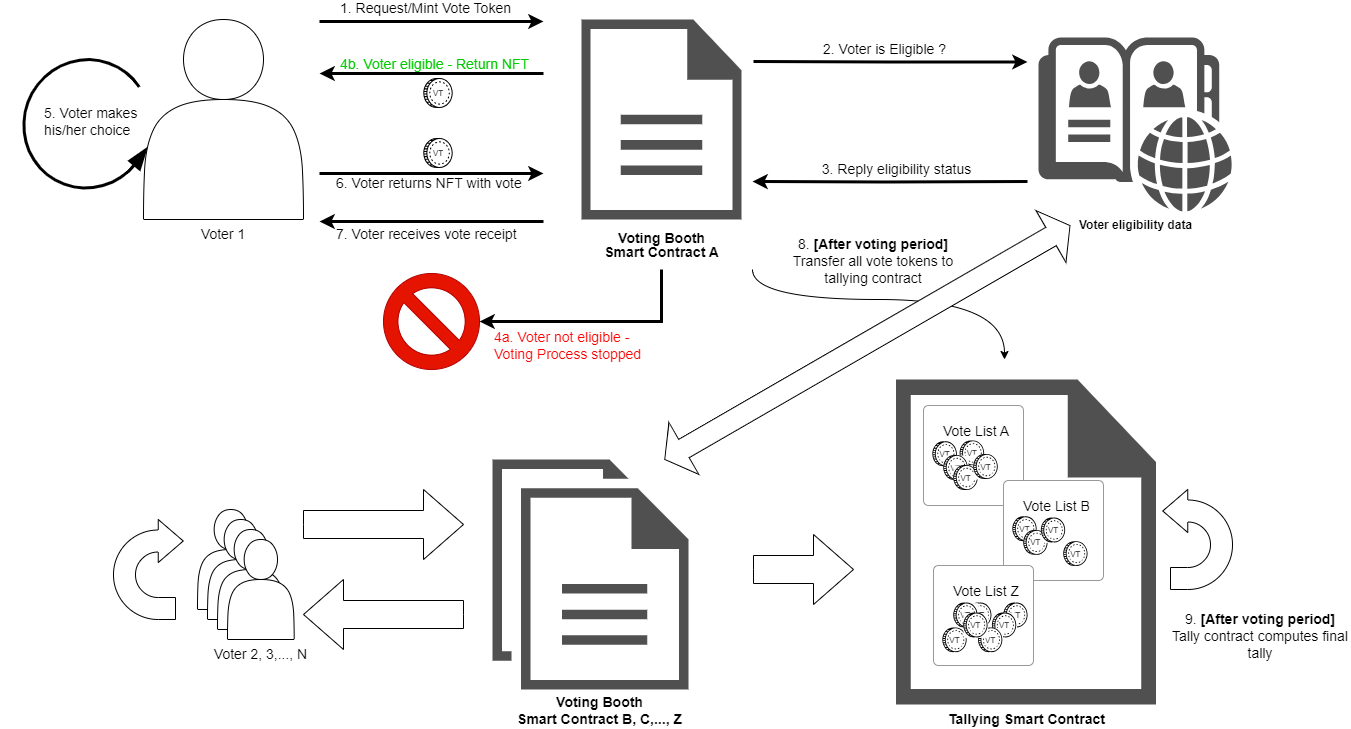
\includegraphics[width=0.7\textwidth]{../Images/01_general_solution.png}
    \caption{General architecture of an NFT based e-voting system.}
    \label{fig:general_architecture}
\end{figure}

The proposed system is not a fully centralised one, as it can be stated from Fig. \ref{fig:general_architecture}, mainly due to the intrinsically restrictive nature of elections, which typically establish \textit{a priori} rules to determine who is eligible to vote or not. The ample nature of these rules (age limit, professional background, nationality, membership in an organisation, etc.) requires the existence of a trusted third party to define and enforce them. Our solution not only does not eliminate this element but also assumes its existence as well as incorporating it into parts of the voting process.

\paragraph{Voting Process}
\begin{enumerate}
    \item{The process begins with a voter interacting with one of the voting booth smart contracts in the available set. Providing multiple points of entry into the system via the creation of multiple but functionally identical voting booth smart contracts increases availability and security by multiplying the effort that an adversary has to endure to prevert the system to his or her favor by a similar factor.
          \par
          The interaction is abstracted by calling a public function in the contract that receives the required inputs from the voter. The process starts by infering over the voter's eligibility to participate in the election.}

    \item{The voting booth smart contract requires a valid eligibility status returned before minting a Vote NFT. The list of eligible voters needs to be provided and managed by an external third party that regulates the election, due to the sensitive nature of most elections. The actual implementation of the authentication step is also a research point identified in this solution. For a detailed explanation of the approaches to consider, please refer to Section \ref{voter_eligibility}, where two potential approaches that achieve the same result are detailed. In each alternative considered, the output from an eligibility query is always a boolean value determining if the voter is allowed to continue.}

    \item{The flow of the process splits in this step depending on the response obtained from the previous one:
          \par
          \textbf{a.} The voter is not eligible for the current election. In this scenario, the process stops, and the voter is informed of the reason for this interruption.
          \par
          \textbf{b.} The voter is cleared for the current election. The voting booth smart contract proceeds with minting a Vote NFT and transferring it to the voter.}

    \item{The voter makes his or her choice by editing the NFT's metadata accordingly. Editing a NFT's metadata is a relatively simple operation, but it still requires a level of technological knowledge that may be out of reach for most people. As such, this step of the process is simplified by abstracting the metadata edition with a contract function. The same function also applies the necessary encryption layers, which are in place to preserve voter privacy as well as to enable the submission of additional votes that replace the previously submitted ones. From a storage point of view, Vote NFTs are stored under the voting booth contracts during the election period, where they can be replaced if the voter changes his or her mind, and move to the tally contract once this period ends. This process also removes the unidirectional link between the voter and his or her submitted NFT, which disables the multiple vote casting feature as well. Please refer to Section \ref{multiple_vote_casting} for additional details on this feature.}

    \item{After submitting his or her choice into the Vote NFT's metadata, the voter returns the token back to the voting boot smart contract. We make no assumptions about the storage location of this token at this point. Any transfer operations should be perceived from a token ownership standpoint.
          \par
          The voting booth smart contract stores all Vote NFTs whose encrypted metadata contains the choice of a voter.}

    \item{The submission of a valid vote triggers the return of a receipt to confirm the success of the operation thus far. This receipt is the hash of the transaction used to return the Vote NFT to the voting booth smart contract.}

    \item{The process described thus far has been replicated through several voting booth smart contracts during the election period. Using smart contracts to establish this mechanism also allows for automatic temporal triggers. These are used to divide the election period from the tally period, using a temporal condition to switch the functionalities available in the voting booth contracts.
          \par
          During the election period, voting booth contracts accept and validate voter requests, as well as process Vote NFTs for successful voter requests. The end of the election period triggers the start of the tally period. During it, voting booth contracts refuse voter requests by default, either to mint a Vote NFT or to submit a previously minted token, while they transfer all stored tokens thus far to a tally contract.
          \par
          With all Vote NFTs are under the control of the tallying smart contract, the counting can begin once the data is ready, i.e., all encryption layers and randomizing elements (salt) are removed from the vote data.
          \par
          Once finished, the final tally is retrieved from this contract through a public function. The tally results remain stored in this contract for future reference and auditing purposes.}
\end{enumerate}

The general approach described morphs into two different systems depending on the type of data storage paradigm employed by the blockchain used to implement this system. Sections \ref{contract-based-approach} and \ref{account-based-approach} detail the two options in greater detail.

\subsection{Contract-based Approach}
\label{contract-based-approach}
\subfile{./05_ContractBasedApproach.tex}

\subsection{Account-based Approach}
\label{account-based-approach}
\subfile{./06_AccountBasedApproach.tex}
\end{document}